% !Mode:: "TeX:UTF-8"

\titlepage

\begin{frame}{说在前面}
	\linespread{1.5}
	  \begin{itemize}[<+-|alert@+>]
	    \item \ba{箭头!箭头!箭头!}
	    \item \ba{画图!画图!画图!}
	    \item \ba{雷同!雷同!雷同!}
% 	    \item 不记得自己哪周交作业
	  \end{itemize}
\end{frame}

% \begin{frame}{需要注意的问题}
% 	\linespread{1.5}
% 	  \begin{itemize}%[<+-|alert@+>]
% 	    \item L'Hospital法则
% 	    \begin{itemize}
% 	      \item \it 只能应用于“$\df{\bm{0}}{\bm{0}}$”
% 	      和“$\df{\bm{\infty}}{\bm{\infty}}$”型
% 	      \item \it 及时使用无穷小代换进行简化
% 	      \item \it 不正规的符号:\b 
% 	      $\xlongequal{\footnotesize\mbox{“L”}}$、
% 	      $\xlongrightarrow{\footnotesize\mbox{“L'Hospital法则”}}$、
% 	      $\df{\bm{0}}{\bm{0}}$、$\df{\bm{\infty}}{\bm{\infty}}$
% 	    \end{itemize}
% 	    \item Taylor公式
% 	    \begin{itemize}
% 	      \item \it Taylor多项式不包含余项
% 	      \item \it 合并同次幂的系数
% 	      \item \it 尽量按照幂次由低到高排列,最后写余项
% 	    \end{itemize}
% 	  \end{itemize}
% \end{frame}

\section{空间曲面}

\begin{frame}
	\linespread{1.5}
	\ba{1.求直线$l:\df{x}{a}=\df{y-b}0=z$绕$z$轴旋转一周所得曲面方程,
	并指出该曲面的类型。}
	
	\bigskip
	
	\small 解:\it
	设$P(x,y,z)$为所求曲面上任意一点,则其必位于直线$l$上某点$Q$绕$z$轴旋转的轨迹上,
	$Q$的坐标可表示为$(at,b,t)$,故必有
	$$\left\{\begin{array}{l}
		x^2+y^2=(at)^2+b^2\\
		z=t
	\end{array}\right.$$
	消去以上两个方程中的$t$,可得
	$$x^2+y^2-a^2z^2=b^2.$$
	即为所求的旋转曲面方程,根据$a,b$取值的不同,其对应的几何对象分别为:
	\begin{enumerate}[(1)]
	  \setlength{\itemindent}{1cm}
	  \item $a=b=0$:$z$轴;
	  \item $a\ne0,b=0$:圆锥面;
	  \item $a\ne0,b\ne0$:单叶双曲面;
	  \item $a=0,b\ne0$:圆柱面。
	\end{enumerate}
	\fin
\end{frame}

\begin{frame}
	\linespread{1.5}
% 	\ba{1.求直线$l:\df{x}{a}=\df{y-b}0=z$绕$z$轴旋转一周所得曲面方程,
% 	并指出该曲面的类型。}
	
% 	\bigskip
	
	\small \it
	旋转曲面方程:
	$$x^2+y^2-a^2z^2=b^2.$$
	根据$a,b$取值的不同,其对应的曲面分别为:
	\begin{enumerate}[(1)]
	  \setlength{\itemindent}{1cm}
	  \item $a=b=0$:$z$轴;
	  \item $a\ne0,b=0$:圆锥面;
	  \item $a\ne0,b\ne0$:单叶双曲面;
	  \item $a=0,b\ne0$:圆柱面。
	\end{enumerate}
	\fin
\end{frame}

\begin{frame}
	\linespread{1.5}
	\ba{2.已知点$A(1,0,0)$与点$B(0,1,1)$,直线$AB$绕$z$轴旋转一周
	所成的旋转曲面为$S$,求$S$与$z=0$、$z=1$所围成的立体体积。}
	\pause

% 	\bigskip
	\small 
	\begin{columns}
		\begin{column}{.4\textwidth}
			\begin{center}
				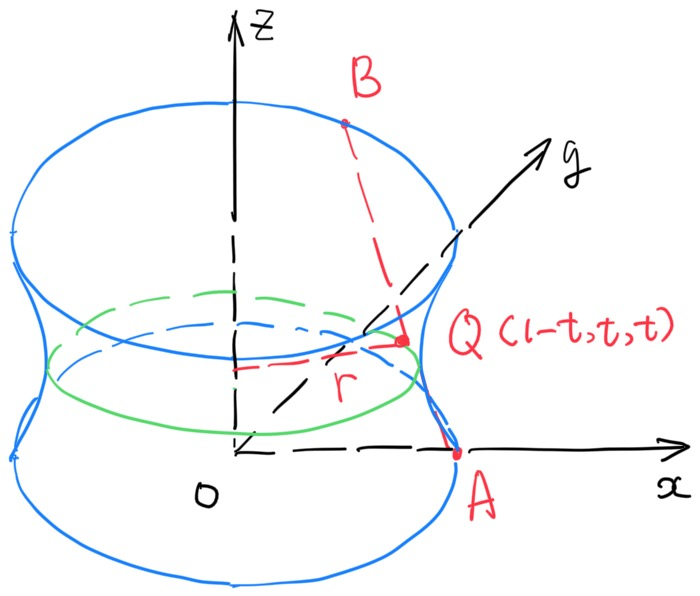
\includegraphics[width=.9\textwidth]{./images/ch8/abzz.jpg}
		% 		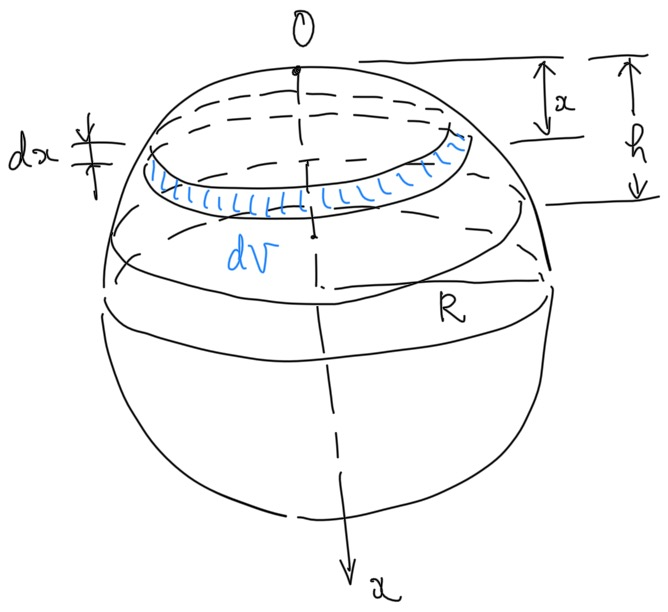
\includegraphics[width=6cm]{./images/ch6/topSp.jpg}
			\end{center}
		\end{column}
		\begin{column}{.6\textwidth}
			解:\it
			则所求立体体积为
			$$V=\dint_0^1\pi r^2\d z.$$
			其中$r$为与$z$对应的$AB$上某点$Q$到$z$轴的距离,注意到
			直线$AB$的参数方程为
			$x=1-t,\quad y=t,\quad z=t$,
			故$r=\sqrt{x^2+y^2}=\sqrt{1-2t+2t^2}$,进而
		\end{column}
	\end{columns}
	$$V=\dint_0^1\pi r^2\d z
	=\dint_0^1\pi(1-2t+2t^2)\d t=\df23\pi.$$
	\fin
\end{frame}

\begin{frame}
	\linespread{1.5}
	\ba{3.设柱面的母线平行于直线$x=y=z$,准线为$xOy$平面内的单位圆
	$x^2+y^2=1$,求柱面的方程。}
	\pause

% 	\bigskip
	\small 
	\begin{columns}
		\begin{column}{.4\textwidth}
			\begin{center}
				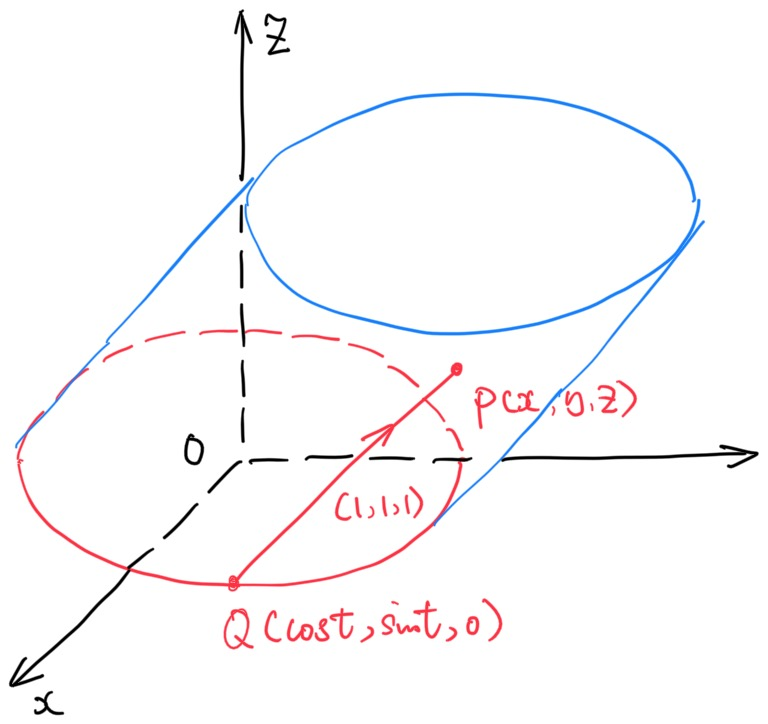
\includegraphics[width=.9\textwidth]{./images/ch8/cpq.jpg}
		% 		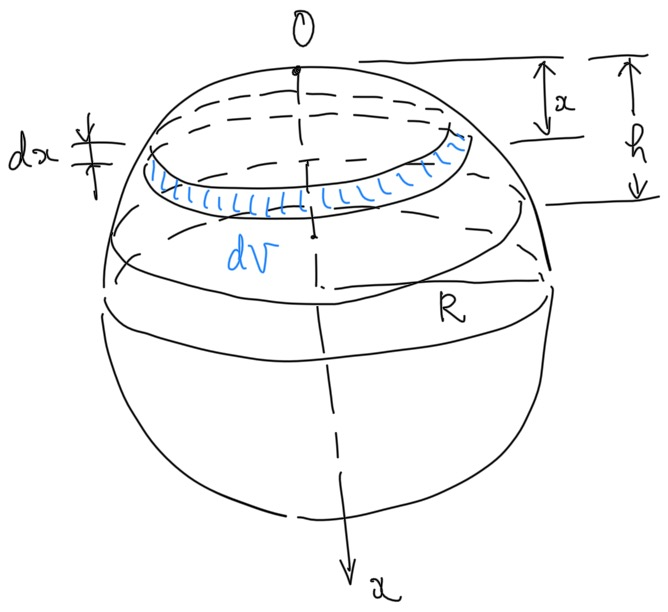
\includegraphics[width=6cm]{./images/ch6/topSp.jpg}
			\end{center}
		\end{column}
		\begin{column}{.6\textwidth}
			解:\it
			设$P(x,y,z)$为所求柱面上任意一点,由柱面的特点可知,其必位于过
			已知单位圆上某点$Q(\cos t,\sin t,0)$且方向平行于$(1,1,1)$的直线上。
			从而可得
			$$\df{x-\cos t}1=\df{y-\sin t}1=\df{z}1,$$
			消去其中的参数$t$,可得
			$$(x-z)^2+(y-z)^2=1,$$
			即为所求柱面的方程。\fin
		\end{column}
	\end{columns}
\end{frame}

\section{空间曲线}

\begin{frame}
	\linespread{1.5}
	\ba{1.一束光线垂直于平面$x+y+z=0$,照射在球面$x^2+y^2+(z-1)^2=1$上,
	求球面在$xOy$平面上的投影的边界曲线方程。}
	
% 	\bigskip
	
	\small 解:\it 如图
	\begin{center}
		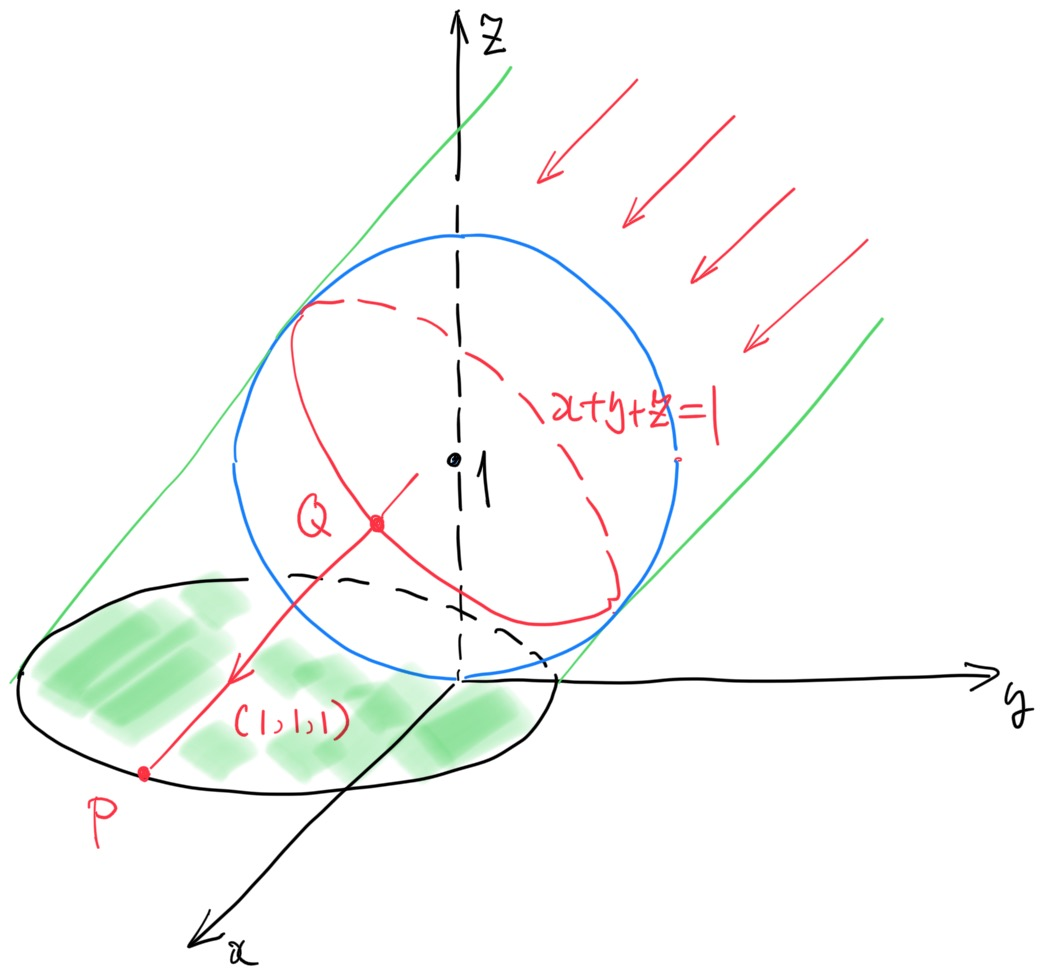
\includegraphics[width=0.5\textwidth]{./images/ch8/sunray.jpg}
	\end{center}
\end{frame}

\begin{frame}
	\linespread{1.5}
% 	\ba{1.一束光线垂直于平面$x+y+z=0$,照射在球面$x^2+y^2+(z-1)^2=1$上,
% 	求球面在$xOy$平面上的投影的边界曲线方程。}
	
% 	\bigskip
	
	\small \it 
	设$P(x,y,0)$为所求边界曲线上一点,由投影柱面的性质,其必位于经过
	球面上某点$Q(x_0,y_0,z_0)$平行于$(1,1,1)$的直线上,由此可知
	$$\df{x-x_0}1=\df{y-y_0}1=\df{-z_0}1.$$
	又显然$Q$位于经过球心且与$(1,1,1)$垂直的平面与球面的交线上,故必有
	$$\left\{\begin{array}{l}
		x_0^2+y_0^2+(z_0-1)^2=1\\
		x_0+y_0+z_0=1
	\end{array}\right.$$
	联立以上所得各方程,消去$x_0,y_0,z_0$,最终可得所求投影边界的曲线方程为
	$$\left\{\begin{array}{l}
		1+x+y+x^2-xy+y^2=\df32\\
		z=0
	\end{array}\right.$$
	\fin
\end{frame}

\begin{frame}
	\linespread{1.5}
	\ba{2.过直线$l:x=y=-z$的平面$\pi$与柱体$x^2+y^2\leq1$
	相交的截面为$S$,求$\pi$的方程,使得$S$的面积最小,并给出$\pi$与柱面$x^2+y^2=1$
	的交线$C$的参数方程。}
	
	\small 解:\it
	如图
	\begin{center}
		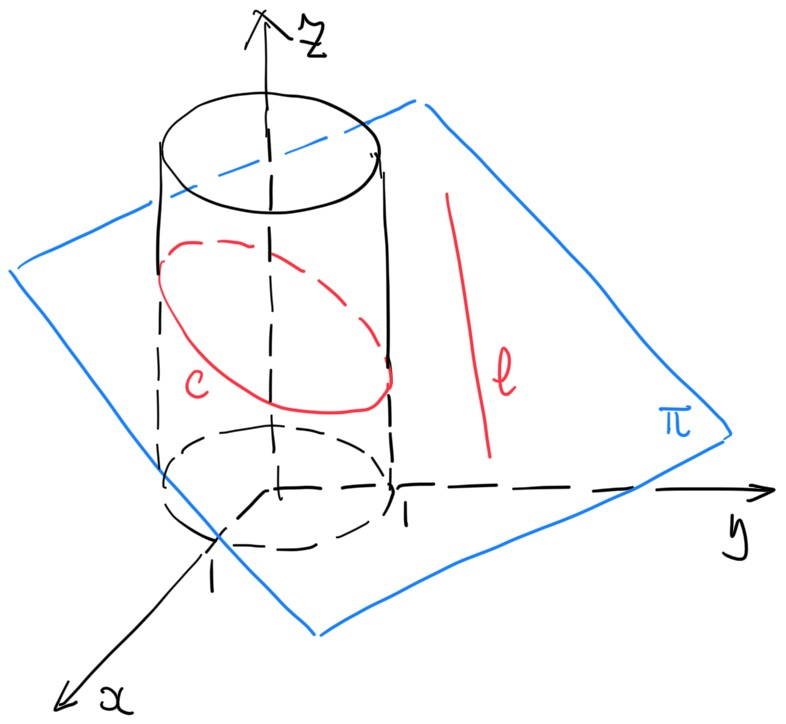
\includegraphics[width=0.5\textwidth]{./images/ch8/ccS.jpg}
	\end{center}
\end{frame}

\begin{frame}
	\linespread{1.5}
	
	\small \it
	设平面$\pi$与$xOy$平面的夹角为$\gamma$,注意到截面$S$在$xOy$平面上的投影为
	单位圆,故必有其面积$A=\df{\pi}{|\cos\gamma|}$,
	显然,当$|\cos\gamma|$取最大值时,截面$S$的面积最小。
	
	由已知,可设过$l$的平面束为
	$$\lambda(x-y)+\mu(x+z)=0,$$
	其方向向量为$\bm{n}=(\lambda+\mu,-\lambda,\mu)$,故
	$$\cos\gamma=\df{\bm{n}\cdot\bm{k}}{|\bm{n}||\bm{k}|}
	=\df{\mu}{\sqrt{2(\lambda^2+\lambda\mu+\mu^2)}}.$$
	不难解得,当$\frac{\lambda}{\mu}=-\df12$时,$|\cos\gamma|$取到最大值$\df{\sqrt6}3$。
	由此,令$\lambda=1,\mu=-2$,可得所求$\pi$的方程为
	$x+y+2z=0$。
\end{frame}

\begin{frame}
	\linespread{1.5}
	
	\small \it
	所求$\pi$的方程为
	$$x+y+2z=0.$$
	相应地曲线$C$可表示为
	$$\left\{\begin{array}{l}
		x^2+y^2=1\\
		x+y+2z=0
	\end{array}\right.$$
	不难求得其参数方程为
	$$\left\{\begin{array}{l}
		x=\cos t\\
		y=\sin t\\
		z=-\df12(\cos t+\sin t)
	\end{array}\right.
	\quad (t\in[0,2\pi])$$
	\fin
\end{frame}

\begin{frame}
	\linespread{1.5}
	\ba{3.画出以下空间区域的图形:	
	(1)曲面$(x-z)^2+y^2=1$与$z=-1,z=1$所围空间区域}
	
	\small 解:
	\begin{center}
		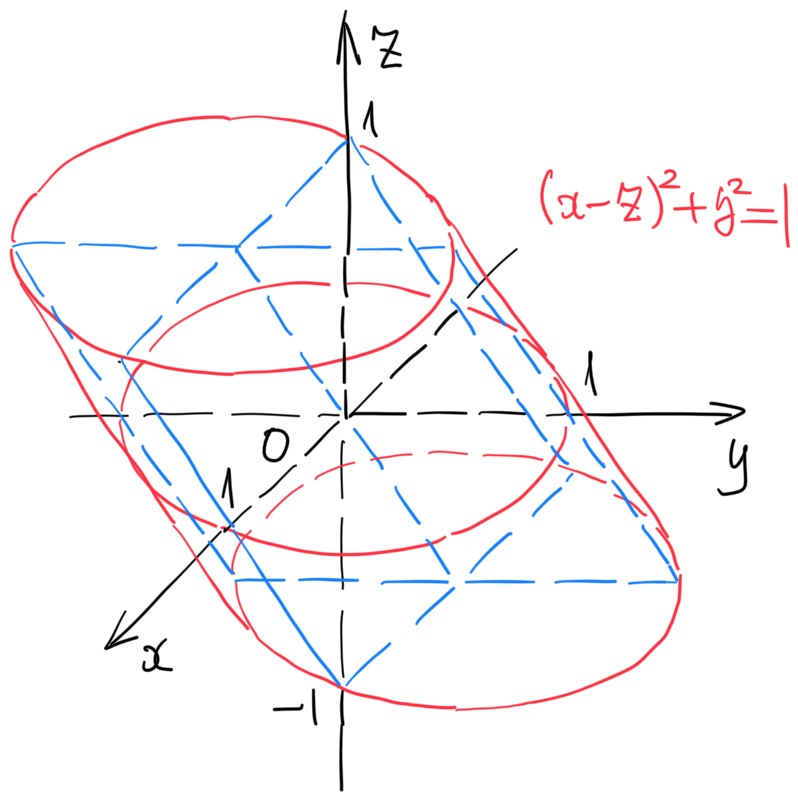
\includegraphics[width=0.5\textwidth]{./images/ch8/xzy-cl.jpg}
	\end{center}
\end{frame}


\begin{frame}
	\linespread{1.5}
	\ba{(2)$0\leq x\leq 1,0\leq y\leq x,0\leq z\leq xy$}
	
	\small 解:	
	\begin{center}
		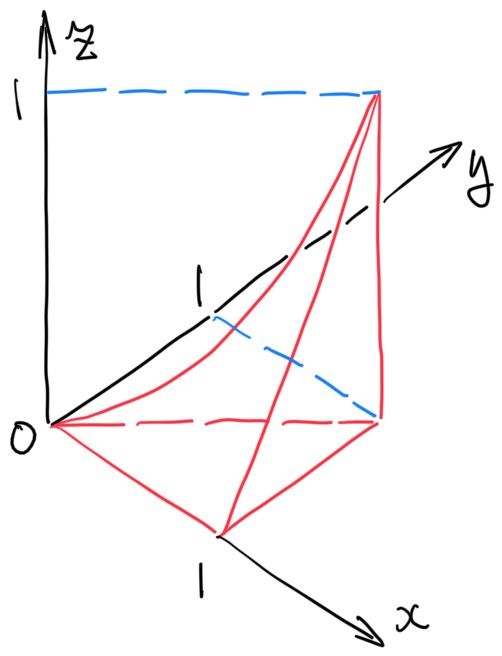
\includegraphics[width=0.4\textwidth]{./images/ch8/3int-1.jpg}\quad\quad
		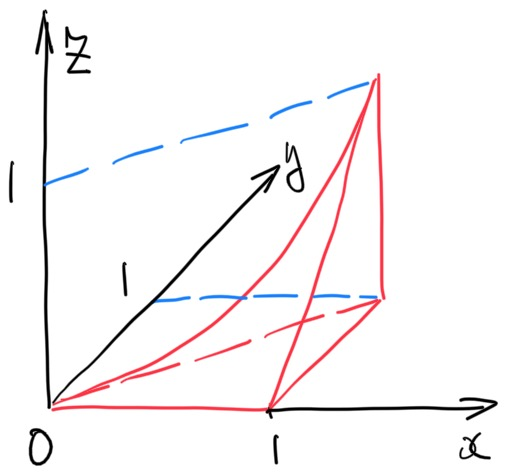
\includegraphics[width=0.45\textwidth]{./images/ch8/3int-2.jpg}
	\end{center}
	\fin
\end{frame}

\section{向量值函数}

\begin{frame}
	\linespread{1.5}
	\ba{1.证明向量值函数的求导法则:
	
	(1)$[\bm{u}(t)\cdot\bm{v}(t)]'
    =\bm{u}'(t)\cdot\bm{v}(t)+\bm{u}(t)\cdot\bm{v}'(t)$
    
    (2)$[\bm{u}(t)\times\bm{v}(t)]'
    =\bm{u}'(t)\times\bm{v}(t)+\bm{u}(t)\times\bm{v}'(t)$ 
    
    进而由此给出并证明三阶行列式
	  $$\left|\begin{array}{ccc}
	  	a_1(t) & a_2(t) & a_3(t)\\
	  	b_1(t) & b_2(t) & b_3(t)\\
	  	c_1(t) & c_2(t) & c_3(t)
	  \end{array}\right|$$
	  的求导法则。	 }
\end{frame}

\begin{frame}
	\linespread{1.5}
	
	\small 解:\it 令$\bm{a}=(a_1(t), a_2(t), a_3(t))$,
	$\bm{b}=(b_1(t), b_2(t), b_3(t))$,$\bm{c}=(c_1(t), c_2(t), c_3(t))$,
	应用以上的求导法则
	\begin{align*}
		&[(\bm{a}\times\bm{b})\cdot\bm{c}]'
		=(\bm{a}\times\bm{b})'\cdot\bm{c}+(\bm{a}\times\bm{b})\cdot\bm{c}'\\
		&=(\bm{a}'\times\bm{b})\cdot\bm{c}+(\bm{a}\times\bm{b}')\cdot\bm{c}
		+(\bm{a}\times\bm{b})\cdot\bm{c}'\\
		&=\left|\begin{array}{ccc}
  	a_1' & a_2' & a_3'\\
  	b_1 & b_2 & b_3\\
  	c_1 & c_2 & c_3
  \end{array}\right|
  +\left|\begin{array}{ccc}
  	a_1 & a_2 & a_3\\
  	b_1' & b_2' & b_3'\\
  	c_1 & c_2 & c_3
  \end{array}\right|
  +\left|\begin{array}{ccc}
  	a_1 & a_2 & a_3\\
  	b_1 & b_2 & b_3\\
  	c_1' & c_2' & c_3'
  \end{array}\right|.
	\end{align*}
	\fin
\end{frame}

\begin{frame}
	\linespread{1.5}
	\ba{2.Newton的万有引力定律可表述为
  $$\bm{F}=-\df{GmM}{r^3}\bm{r},$$
  其中$m$和$M$分别为行星和太阳的质量,$r$表示两者(球心)之间的距离,
  $\bm{r}$为由太阳中心指向行星中心的向量。
  \begin{enumerate}[(1)]
%     \setlength{\itemindent}{1cm}
    \item 求行星运动的加速度$\bm{r}''$;
    \item 证明行星总是运行在一个经过太阳中心的平面内,也即
    $\bm{r}\times\bm{r}'$为常向量。
  \end{enumerate}}
\end{frame}

\begin{frame}
	\linespread{1.5}
	\small 解:\it (1)由Newton第二定律,
	$$\bm{r}''=\df{\bm{F}}{m}=-\df{GM}{r^3}\bm{r}.$$
	
	(2)由向量值函数叉乘的求导法则,
	$$
		(\bm{r}\times\bm{r}')'
		=\bm{r}'\times\bm{r}'+\bm{r}\times\bm{r}''
		=\bm{r}\times\bm{r}''=-\bm{r}\times\df{GM}{r^3}\bm{r}=0,
	$$
	由此即知$\bm{r}\times\bm{r}'$为常向量。\fin
	
	\ba{注:本题等价于证明地球转动的角动量守恒,因此不能用角动量守恒来证明以上结论。}
\end{frame}

% \begin{frame}{出现的问题}
% 	\linespread{1.5}
% 	  \begin{itemize}%[<+-|alert@+>]
% 	    \item 作业进度慢!
% 	    \item 概念问题
% 	    \begin{itemize}
% 	      \item \b\it 幂级数展开不熟练
% 	      \item \b\it Maclaurin级数和关于$(x-x_0)$的幂级数分不清
% 	    \end{itemize}
% 	    \item 过程不规范或不完整
% 	    \begin{itemize}
% 	      \item \b\it 求收敛域要单独讨论端点的敛散性
% 	      \item \b\it 相同幂次的项要合并,并按幂次从小到大排列
% 	      \item \b\it 书写潦草随意\pause
% 	    \end{itemize}
% 	    \item \ba{雷同!!!}
% 	  \end{itemize}
% \end{frame}

% \begin{frame}
% 	\linespread{1.5}
% 	\ba{3.设$D$是由曲线$y=\sin x+1$与三条直线$x=0,x=\pi,y=0$
% 	所围成的曲边梯形,求$D$绕$x$轴旋转一周所围成的旋转体的体积。
% 	}
% 	\pause
% 	
% % 	\bigskip
% 	
% 	\begin{columns}
% 		\begin{column}{.5\textwidth}
% 			\begin{center}
% 				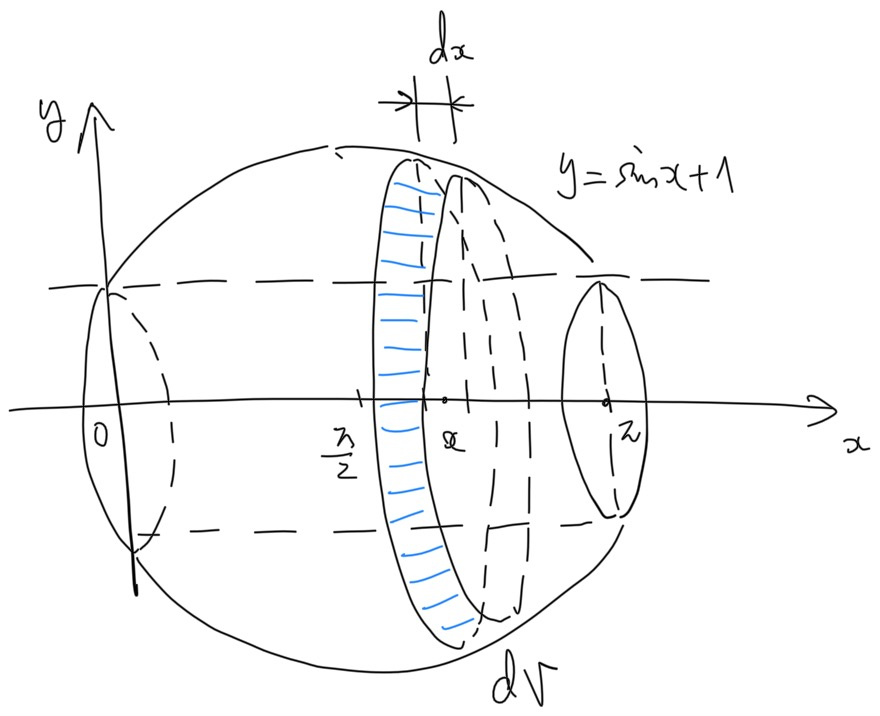
\includegraphics[width=.9\textwidth]{./images/ch6/sinx1cs.jpg}
% 		% 		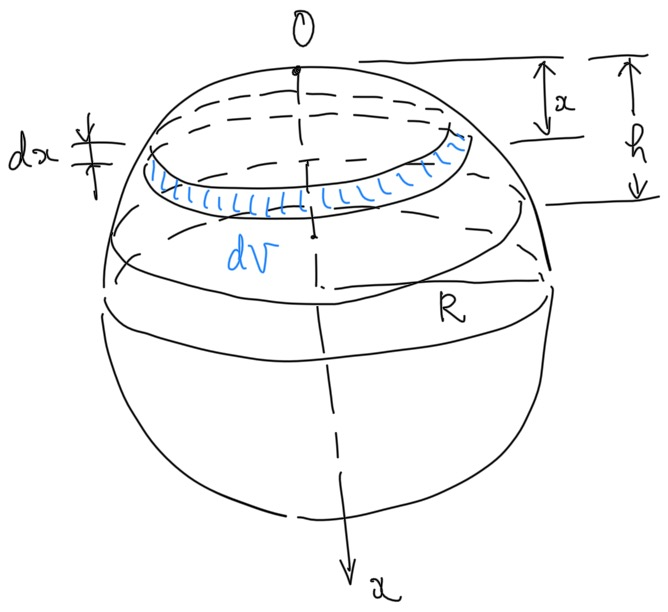
\includegraphics[width=6cm]{./images/ch6/topSp.jpg}
% 			\end{center}		
% 		\end{column}
% 		\begin{column}{.5\textwidth}
% 			\small 解:\it
% 			如图,体积微元$\d V=\pi y^2\d x$,	故所求体积
% 			$$
% 				V=\dint_0^{\pi}\pi(\sin x+1)^2\d x=\df32\pi^2.
% 			$$
% 		\end{column}
% 	\end{columns}
% \end{frame}